\documentclass[aps,prb,onecolumn,nofootinbib,superscriptaddress]{revtex4-2}
\usepackage{amsmath,amssymb,amsthm,mathtools,bm}
\usepackage{booktabs,graphicx}
\usepackage[colorlinks=true,linkcolor=blue,citecolor=blue,urlcolor=blue]{hyperref}
\usepackage{microtype}
\newcommand{\bk}{\boldsymbol{k}}
\newcommand{\bd}{\boldsymbol{d}}
\newcommand{\br}{\boldsymbol{r}}
\newcommand{\bq}{\boldsymbol{q}}
\newcommand{\Id}{\mathbf{1}}
\newcommand{\ii}{\mathrm{i}}
\newcommand{\BZ}{\mathrm{BZ}}
\newcommand{\Chern}{\mathcal{C}}
\newcommand{\avg}[1]{\left\langle #1\right\rangle_{\BZ}}
\DeclareMathOperator{\tr}{tr}
\DeclareMathOperator{\sgn}{sgn}
\begin{document}
\title{Finite-range Wannier truncation: band mixing and a five-cell topological parent}
\author{Asadullah Bhuiyan}
\date{October 7, 2026}
\begin{abstract}
We examine what remains of the overcomplete Wannier construction after its spatial support is truncated. The overlap with the target band still carries the form-factor obstruction, but the truncated mode also acquires weight in the opposite band. These are different statements: the persistence of an overlap zero does not by itself imply that a parent Hamiltonian remains topological. We derive the signed parent generated by the truncated modes and compare the usual nine-cell square with the five-cell plus obtained by removing its corners. At $\alpha=1$, the plus parent reduces to a nearest-neighbor QWZ Hamiltonian with renormalized coefficients. It remains gapped with occupied-band Chern number $1$, and the corners can be removed continuously without closing the gap. We also identify the cost of this smaller support: greater band mixing and an earlier parent-band transition. Finally, we specify the sense in which the plus is minimal under fourfold rotation and distinguish these reference-band statements from the topology of a conditioned circuit trajectory.
\end{abstract}
\maketitle
\setcounter{tocdepth}{2}
\tableofcontents

\section{The target band and its OW modes}

We use the two-band model
\begin{equation}
 h_{\rm QWZ}(\bk)=\boldsymbol{n}(\bk)\cdot\boldsymbol{\sigma},
 \qquad \boldsymbol{n}(\bk)=(\sin k_x,\sin k_y,\alpha-\cos k_x-\cos k_y),
 \qquad P_\pm(\bk)=\frac{\Id\pm\widehat{\boldsymbol{n}}(\bk)\cdot\boldsymbol{\sigma}}{2}.
 \label{eq:model}
\end{equation}
Here $\widehat{\boldsymbol{n}}=\boldsymbol{n}/|\boldsymbol{n}|$, and the lower band has $\Chern=1$ for $0<\alpha<2$ in our convention~\cite{Qi2006}. Unless stated otherwise, we set $\alpha=1$. We write $\avg{X}=\int_{\BZ}d^2\bk\,X/(2\pi)^2$ and choose the orthonormal trial orbitals $\tau_A=(1,1)^{\mathsf T}/\sqrt{2}$ and $\tau_B=(1,-1)^{\mathsf T}/\sqrt{2}$.

The OW construction projects each translated trial orbital into a band and normalizes it~\cite{BPJ,Li2024}. With the Fourier convention
\begin{equation}
 P_\pm(\bd)=\avg{e^{\ii\bk\cdot\bd}P_\pm(\bk)},
 \qquad
 W_{\br,\nu,\pm}(\br')=\frac{P_\pm(\br'-\br)\tau_\nu}{\sqrt{Z_\infty}},
 \qquad Z_\infty=\avg{\langle\tau_\nu|P_\pm|\tau_\nu\rangle}=\frac12,
 \label{eq:ow}
\end{equation}
each mode has unit real-space norm. The last equality follows from reflection symmetry: the Brillouin-zone average of $\widehat n_x$ vanishes. Since $\sum_\nu|\tau_\nu\rangle\langle\tau_\nu|=\Id$, summing both families and all translations gives
\begin{equation}
 \sum_{\br,\nu}|W_{\br,\nu,-}\rangle\langle W_{\br,\nu,-}|=2P_-.
 \label{eq:tight}
\end{equation}
Thus, two OW families reconstruct the occupied projector even though the modes are not mutually orthogonal. At a momentum where one family vanishes, the other supplies the missing direction. This is an overcomplete frame, not an orthonormal Wannier basis.

For a normalized mode, let $\hat\chi^\dagger_{\br,\nu,\pm}=\sum_i W_{\br,\nu,\pm}(i)\hat c_i^\dagger$ and $\hat{\mathcal N}_{\br,\nu,\pm}=\hat\chi^\dagger_{\br,\nu,\pm}\hat\chi_{\br,\nu,\pm}$. The ideal half-filled Slater determinant occupies every lower-band mode and empties every upper-band mode. All of these conditions are compatible before truncation, despite the nonorthogonality within a band. Our question is what survives when each measurement mode is confined to a few unit cells.

\section{Truncation, overlap zeros, and band mixing}

\subsection{A window changes more than the form factor}

Let $g(\bd)$ be a real window. The usual square choice is $g_w(\bd)=1$ for $|d_x|,|d_y|\le w$ and zero otherwise, where the integer $w=n_{\rm shell}$ is the OW truncation range. Thus, $w=1$ retains nine unit cells. More generally, we assume for now that $g(0)=1$ and the window is inversion symmetric. We define
\begin{equation}
 F_g(\bk)=\sum_{\bd}g(\bd)P_-(\bd)e^{-\ii\bk\cdot\bd},
 \qquad
 |\phi_{\nu,-;g}(\bk)\rangle=\frac{F_g(\bk)|\tau_\nu\rangle}{\sqrt{Z_{\nu,-;g}}},
 \qquad
 Z_{\nu,-;g}=\sum_{\bd}g(\bd)^2\|P_-(\bd)\tau_\nu\|^2.
 \label{eq:window}
\end{equation}
The normalization is over real space, or equivalently over the entire Brillouin zone. We do not normalize $\phi$ independently at each momentum. Also, $F_g$ is Hermitian, but it is generally not a projector.

Writing $\widetilde g(\bq)=\sum_{\bd}g(\bd)e^{-\ii\bq\cdot\bd}$, with $\bq$ a momentum difference, gives the convolution
\begin{equation}
 |\phi_{\nu,-;g}(\bk')\rangle
 =\frac{1}{\sqrt{Z_{\nu,-;g}}}\int_{\BZ}\frac{d^2\bk}{(2\pi)^2}
 \widetilde g(\bk'-\bk)|u_-(\bk)\rangle\langle u_-(\bk)|\tau_\nu\rangle.
 \label{eq:convolution}
\end{equation}
The eigenvector $u_-$ is understood in local gauges; the projector and the full integrand are gauge independent. Taking the overlap with $u_-(\bk')$ introduces $\langle u_-(\bk')|u_-(\bk)\rangle$. Taking the overlap with $u_+(\bk')$ instead introduces $\langle u_+(\bk')|u_-(\bk)\rangle$, which need not vanish when $\bk\ne\bk'$. Truncation therefore both deforms the in-band form factor and mixes the bands.

The effective form factor $f^{\rm eff}_{\nu,-;g}(\bk)=\langle u_-(\bk)|\phi_{\nu,-;g}(\bk)\rangle$ cannot be smooth and nonzero everywhere for a Chern band. More precisely, its projected section $P_-\phi$ must have zeros. For isolated zeros, the sum of their local counterclockwise phase windings is $-\Chern$~\cite{BPJ}. At $\alpha=1$, the lower-band $A$-family has its untruncated winding-$(-1)$ zero at $(k_x,k_y)=(\pi/2,0)$. The zero moves to $k_x/\pi\simeq0.492186$ for the nine-cell square and to $0.487864$ for the plus, retaining winding $-1$ in both cases.

This is a statement about the overlap with the \emph{target band}. It is not the Chern number of an individual truncated mode, nor is it a test of the occupied band of a new Hamiltonian. The onsite window makes the distinction particularly clear: its effective form factor still has a winding-$(-1)$ zero, even though its parent is momentum independent and topologically trivial. Local windings are stable under deformations that keep the overlap nonzero on the loop boundary; no holomorphic assumption is needed.

\subsection{Band mixing frustrates the exact stabilizing conditions}

For each normalized mode we quantify opposite-band weight by
\begin{equation}
 \epsilon_g=\avg{\langle\phi_{\nu,-;g}|P_+|\phi_{\nu,-;g}\rangle}.
 \label{eq:leakage}
\end{equation}
The upper-band definition exchanges $+$ and $-$. The values agree for all four family/band choices for the windows considered here. At $\alpha=1$, we find $\epsilon_g\simeq0.00395$ for the nine-cell square and $0.02553$ for the plus. The plus still retains $95.14\%$ of the original OW norm, but its band mixing is appreciably larger than that of the square. Retained norm and opposite-band weight measure different things and should not be interchanged.

Band mixing also removes exact linear dependence among translated modes. On an $8\times8$ torus, the 128 untruncated lower-band modes have rank 64. Rebuilding the projector on that torus and then truncating gives rank 128 for the plus and for squares of range $w=1,2$. The upper families have the same ranks. The smallest singular value of the normalized synthesis matrix is approximately $0.0449$ for the plus and $0.00117$ for the range-one square. Thus, filling every truncated lower-band mode would fill the entire single-particle space, which is incompatible with emptying the upper-band modes. The exact stabilizing conditions become frustrated. We will see that this does not force the auxiliary parent to lose its topological band.

\begin{figure}[tb]
 \centering
 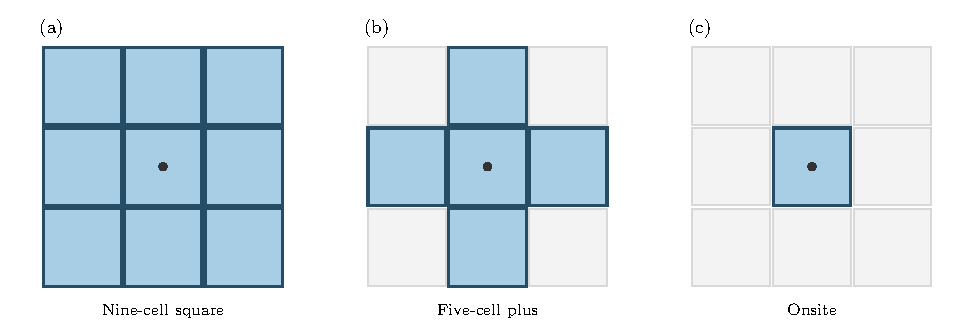
\includegraphics[width=6.5in]{figures/support_windows.pdf}
 \caption{\textbf{Spatial windows.} The nine-cell square, five-cell plus, and onsite support. Colored cells are retained; both physical orbitals in each retained unit cell are included. The dot marks the center. The square and plus both retain fourfold rotation symmetry of the support.}
 \label{fig:support}
\end{figure}

\section{The signed parent and its occupied band}

For the reflection-symmetric windows in Fig.~\ref{fig:support}, the normalization in Eq.~\eqref{eq:window} is common to the two families and two bands; call it $Z_g$. Since $P_+(\bd)=\delta_{\bd,0}\Id-P_-(\bd)$,
\begin{equation}
 |\phi_{\nu,+;g}\rangle=\frac{(\Id-F_g)|\tau_\nu\rangle}{\sqrt{Z_g}},
 \quad
 S_{-,g}=\sum_\nu|\phi_{\nu,-;g}\rangle\langle\phi_{\nu,-;g}|=\frac{F_g^2}{Z_g},
 \quad
 S_{+,g}=\frac{(\Id-F_g)^2}{Z_g}.
\end{equation}
We use the \emph{signed} parent, not the lower-frame operator alone:
\begin{equation}
 h_g=S_{+,g}-S_{-,g}=\frac{\Id-2F_g}{Z_g},
 \qquad R_g=\mathbf{1}_{(1/2,\infty)}(F_g).
 \label{eq:parent}
\end{equation}
Here $R_g$ is the occupied spectral projector. The quadratic terms cancel between gain and loss families. Writing $F_g=(\Id-\boldsymbol d_g\cdot\boldsymbol\sigma)/2$, reflection symmetry gives
\begin{equation}
 Z_g=\frac{1+\avg{|\boldsymbol d_g|^2}}{4}.
 \label{eq:norm}
\end{equation}
Indeed, $F_g^2=[(1+|\boldsymbol d_g|^2)\Id-2\boldsymbol d_g\cdot\boldsymbol\sigma]/4$, the trial orbitals have zero $\sigma^y,\sigma^z$ expectation, and $\avg{d_{g,x}}=0$.

There is a simple sufficient condition for this parent to remain in the target phase. If
\begin{equation}
 \delta_g=\sup_{\bk}\|F_g(\bk)-P_-(\bk)\|_{\rm op}<\frac12,
 \label{eq:error}
\end{equation}
then the eigenvalues of $F_s=P_-+s(F_g-P_-)$, $0\le s\le1$, cannot cross $1/2$. Its rank-one spectral projector above $1/2$ therefore interpolates smoothly between $P_-$ and $R_g$. The Chern number is unchanged along this gapped path~\cite{Avron1983}. Moreover,
\begin{equation}
 \Delta_0(g)\equiv\min_{\bk,n}|E_n[h_g(\bk)]|
 \ge\frac{1-2\delta_g}{Z_g}.
 \label{eq:gapbound}
\end{equation}
Throughout this note, $\Delta_0$ means the distance from zero to the nearest band. The full separation between the occupied and empty bands is $2\Delta_0$, since $h_g$ is traceless. The untruncated values are $\Delta_0=2$ and full gap $4$.

Absolute summability of the gapped projector kernel gives the additional bound
\begin{equation}
 \delta_g\le\sum_{\bd}|1-g(\bd)|\,\|P_-(\bd)\|_{\rm op}.
\end{equation}
For growing square windows this tends to zero, establishing a sufficient large-window condition. At small range we report converged numerical checks, not an interval-certified infinite-tail bound. At $\alpha=1$, sampled values are $\delta_{w=1}\simeq0.098754$ and $\delta_{\rm plus}\simeq0.278594$, both comfortably below $1/2$. Neither a small integrated leakage nor a large retained norm alone establishes this uniform inequality.

The finite range of $h_g$ does not make $R_g$ finite range. Spectral projection restores spatial tails, so this construction does not furnish a compactly supported spanning frame for an isolated Chern band~\cite{DubailRead2015}. In particular, the truncated measurement modes themselves do not lie exactly in the occupied band of $h_g$.

\begin{table}[tb]
 \caption{\textbf{Window comparison at $\alpha=1$.} Retained probability $p_g=Z_g/Z_\infty=2Z_g$, opposite-band weight $\epsilon_g$, position of the winding-$(-1)$ zero of the lower $A$-family overlap, parent half-gap, and occupied-band Chern number. Each real-space mode is normalized before constructing the parent. Gap minima other than the analytically reduced plus result are sampled values.}
 \label{tab:comparison}
 \begin{ruledtabular}
 \begin{tabular}{lrrrrrr}
 Window & Cells & $p_g$ & $\epsilon_g$ & $k_{x,0}/\pi$ & $\Delta_0$ & $\Chern[R_g]$ \\
 Onsite & 1 & 0.620624 & 0.306 & 0.209346 & 1.582825 & 0 \\
Plus & 5 & 0.951417 & 0.0255 & 0.487864 & 0.930845 & 1 \\
Square $w=1$ & 9 & 0.992155 & 0.00395 & 0.492186 & 1.802426 & 1 \\
Square $w=2$ & 25 & 0.999137 & 0.000432 & 0.492488 & 1.902788 & 1 \\
Square $w=4$ & 81 & 0.999979 & 1.07e-05 & 0.499202 & 1.978048 & 1 \\

 \end{tabular}
 \end{ruledtabular}
\end{table}

\section{Removing the corners: the five-cell plus}

\subsection{A nearest-neighbor parent with renormalized coefficients}

We now retain only
\begin{equation}
 \mathcal S_{\rm plus}=\{(0,0),(1,0),(-1,0),(0,1),(0,-1)\}.
\end{equation}
Parity of the components in Eq.~\eqref{eq:model} fixes the windowed vector to
\begin{equation}
 h_{\rm plus}(\bk)=\frac{1}{Z_{\rm plus}}
 \left[a\sin k_x\,\sigma^x+a\sin k_y\,\sigma^y+
 \bigl(b-c\cos k_x-c\cos k_y\bigr)\sigma^z\right],
 \label{eq:plus}
\end{equation}
where
\begin{equation}
 a=2\avg{\widehat n_x\sin k_x},\qquad
 b=\avg{\widehat n_z},\qquad
 c=-2\avg{\widehat n_z\cos k_x},\qquad
 Z_{\rm plus}=\frac{1+a^2+b^2+c^2}{4}.
 \label{eq:abc}
\end{equation}
Thus, the signed parent returns to the nearest-neighbor QWZ form, with renormalized parameters. Each individual frame operator can contain longer-range products; those terms cancel in their signed difference. At $\alpha=1$, numerical Brillouin-zone integration gives
\begin{equation}
 a=0.665963659,\qquad b=0.491169158,\qquad c=0.466990149,
 \qquad Z_{\rm plus}=0.475708634.
 \label{eq:abcvalues}
\end{equation}

Since $a\ne0$, a band touching requires $\sin k_x=\sin k_y=0$. The four Dirac masses are
\begin{equation}
 m_\Gamma=b-2c=-0.442811139,\qquad
 m_X=m_Y=b=0.491169158,\qquad
 m_M=b+2c=1.425149455.
 \label{eq:masses}
\end{equation}
Their signs give
\begin{equation}
 \Chern[R_{\rm plus}]=-\frac12\left[\sgn(b-2c)-2\sgn b+\sgn(b+2c)\right]=1.
 \label{eq:diracchern}
\end{equation}
Equivalently, $0<b/c<2$ and $a/c>0$, so we can deform the positive velocity ratio $a/c$ to unity without closing a gap. We are in the same phase as the target, not merely close to it in an averaged sense.

We can also locate the global gap minimum without an unresolved momentum-grid minimum. Set $u=\cos k_x$, $v=\cos k_y$. Then
\begin{equation}
 Z_{\rm plus}^2E(\bk)^2=a^2(2-u^2-v^2)+[b-c(u+v)]^2.
\end{equation}
Because $a^2-c^2\simeq0.225428>0$, this expression is concave in either variable with the other held fixed. Its minimum over $[-1,1]^2$ is therefore at a vertex. Comparing the four masses yields
\begin{equation}
 \Delta_0({\rm plus})=\frac{2c-b}{Z_{\rm plus}}=0.930845285,
 \qquad 2\Delta_0({\rm plus})=1.861690570.
 \label{eq:plusgap}
\end{equation}
The coefficient integrals are numerical, but the reduction of the momentum minimization is analytic. The inequalities selecting this phase and minimum have large margins.

\subsection{A continuous path from square to plus}

To check the effect of removing corners directly, let their amplitude be $\lambda$, while the center and four axial neighbors retain amplitude one. The endpoints $\lambda=1$ and $0$ are the square and plus. Real-space normalization gives
\begin{equation}
 F_\lambda=F_{\rm plus}+\lambda(F_\square-F_{\rm plus}),\qquad
 Z_\lambda=Z_{\rm plus}+\lambda^2(Z_\square-Z_{\rm plus}).
 \label{eq:path}
\end{equation}
The dependence on $\lambda^2$ in the norm matters: we reduce amplitudes before renormalizing each mode. Fourier symmetry gives
\begin{align}
 Z_\lambda h_\lambda(\bk)={}&(a+\lambda d\cos k_y)\sin k_x\,\sigma^x
 +(a+\lambda d\cos k_x)\sin k_y\,\sigma^y\nonumber\\
 &+\left[b-c(\cos k_x+\cos k_y)+\lambda e\cos k_x\cos k_y\right]\sigma^z,
 \label{eq:pathharmonics}
\end{align}
with $d=4\avg{\widehat n_x\sin k_x\cos k_y}=0.232187855$ and
$e=4\avg{\widehat n_z\cos k_x\cos k_y}=-0.466990149$ at $\alpha=1$.
Since $a>|d|$, the sine prefactors cannot vanish for $0\le\lambda\le1$. Possible closings are again restricted to the four high-symmetry momenta. Their masses are
\begin{equation}
 b-2c+\lambda e<0,\qquad b-\lambda e>0,\qquad b+2c+\lambda e>0
 \quad (0\le\lambda\le1).
\end{equation}
No mass crosses zero. Thus, the corners can be removed continuously at fixed Chern number. Figure~\ref{fig:corners}(b) shows the normalized gap along this path: it decreases toward the plus endpoint but does not close.

\begin{figure}[tb]
 \centering
 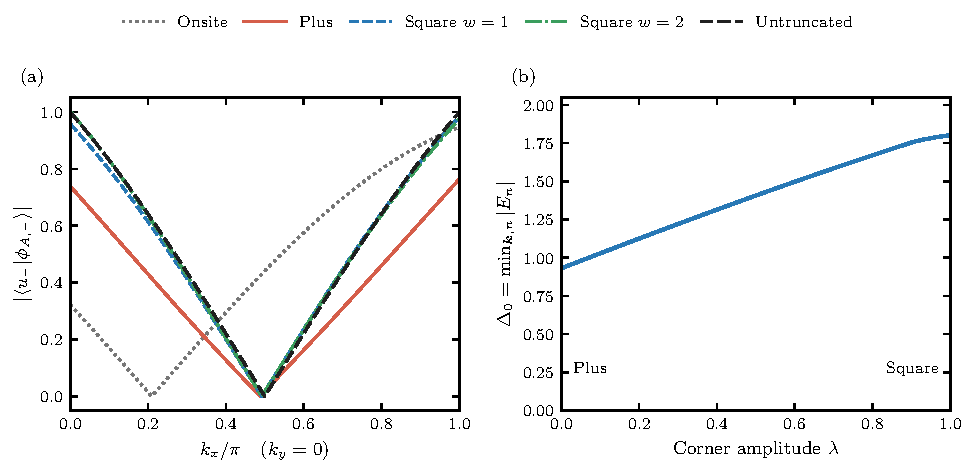
\includegraphics[width=6.5in]{figures/mixing_and_corner_removal.pdf}
 \caption{\textbf{Overlap deformation and corner removal at $\alpha=1$.} (a) Target-band overlap along $k_y=0$, with each OW mode normalized in real space. Even onsite truncation retains an overlap zero; this alone does not determine the parent topology. (b) Parent half-gap as the corner amplitude varies from zero (plus) to one (square). Modes are renormalized at every amplitude. The full band separation is twice the plotted quantity.}
 \label{fig:corners}
\end{figure}

\subsection{The smaller support narrows the parent topological regime}

The plus is not equivalent to the square at every $\alpha$. Its coefficients depend on the target parameter through the integrals in Eq.~\eqref{eq:abc}. The positive-$\alpha$ closing near the original transition occurs when $b(\alpha)=2c(\alpha)$. Solving this equation gives
\begin{equation}
 \alpha_c({\rm plus})\simeq1.500068,
 \qquad\alpha_c(\square,w=1)\simeq1.800138,
 \qquad\alpha_c(\square,w=2)\simeq1.930755,
 \qquad\alpha_c(\square,w=4)\simeq1.979273.
 \label{eq:transitions}
\end{equation}
We checked the occupied-band Chern number on either side of each closing. These are transitions of the signed auxiliary parents; the original QWZ target still changes phase at $\alpha=2$. The square-window drift is consistent with the previously observed empirical behavior $2-\alpha_c(w)\simeq0.40/(w+0.42)^2$ for $w\ge3$. We do not infer a new asymptotic law from the four values in Eq.~\eqref{eq:transitions}.

The distinction is practical. At $\alpha=1$ the corners are unnecessary for the parent topology. Closer to the target transition, their removal can change the phase. The plus also has a smaller gap and larger occupation mismatch with the target band. Its sampled minimum target-band overlap is $\min_{\bk}\tr[P_-R_{\rm plus}]\simeq0.98893$: the reference band remains close to the target, but the measurement modes themselves still have the larger leakage quantified above.

\section{Fourfold symmetry and the sense of minimal support}

The square and plus both have $C_4$ rotation symmetry: a rotation by $90^\circ$ maps either support onto itself. Nine and five count unit cells, not rotation orders. Including reflections, the geometric masks have the square point group $D_4$ (also denoted $C_{4v}$). This is a statement about the \emph{window}, not a claim that a Chern Hamiltonian has every ordinary unitary mirror symmetry of that window. In particular, an orientation-reversing unitary mirror would reverse its Chern number.

For the parent, fourfold covariance includes an orbital rotation:
\begin{equation}
 U_4=e^{-\ii\pi\sigma^z/4},\qquad
 h(-k_y,k_x)=U_4h(k_x,k_y)U_4^\dagger.
\end{equation}
An individual OW family, or an individual ordered measurement record, need not be invariant under this transformation. Removing corners does not lower the rotation symmetry of the parent or the support.

Within the five-cell plus, the axial neighbors form one four-site orbit under $C_4$. Keeping the center and this symmetry leaves only two nonempty choices: all five cells, or the center alone. The onsite parent has
\begin{equation}
 F_0=\frac{\Id-b\sigma^z}{2},\qquad
 h_0=\frac{b}{Z_0}\sigma^z,\qquad Z_0=\frac{1+b^2}{4}.
\end{equation}
It is gapped at $\alpha=1$ but trivial. There is one other nonempty $C_4$-invariant submask: the four arms without the center. For any common window with $g(0)=0$, the identity contribution in $P_+=\Id-P_-$ is removed. The unnormalized upper and lower modes then differ only by a minus sign. Their norms agree pairwise, and consequently
\begin{equation}
 S_{+,g}=S_{-,g},\qquad h_g=0.
 \label{eq:nocenter}
\end{equation}
Thus, no proper nonempty $C_4$-invariant submask of this plus gives a gapped topological signed parent with the same two trial families and both band targets. This is the precise minimality statement. It is not a general lower bound on the number of unit cells required by a topological measurement construction: asymmetric windows or a different construction are outside this argument.

\section{What this says about the adaptive circuit}

The target projector $P_-$, the windowed matrix $F_g$, the auxiliary occupied projector $R_g$, and the actual conditioned-state projector are distinct objects. For a pure number-conserving Gaussian trajectory we write
\begin{equation}
 (G_{\boldsymbol m})_{ij}=\operatorname{Tr}(\hat\rho_{\boldsymbol m}\hat c_i^\dagger\hat c_j),
 \qquad\Gamma_{\boldsymbol m}=G_{\boldsymbol m}^{\mathsf T}.
\end{equation}
Here the transpose converts the stored two-point-function ordering to the spectral-projector ordering used throughout this note.

The signed parent has a direct relation to the occupation penalties: up to a constant, the quadratic form associated with the sum of lower-mode hole penalties and upper-mode particle penalties is $\hat c^\dagger h_g\hat c$. This explains why its half-filled ground state is a useful reference. It does not identify a measurement record with imaginary-time evolution under that Hamiltonian. The strong conditioned updates do not generally commute, their probabilities depend on the current state, and feedback can change the trajectory charge~\cite{BPJ}. Truncation also frustrates the exact mode-by-mode stabilizing conditions, as the rank calculation above demonstrates.

We have therefore established a specific reference-band result: at $\alpha=1$, the signed parent remains in the target phase after removing all four corner cells, and there is an explicit gapped path connecting the square and plus constructions. This makes the plus a natural shorter-range candidate for the circuit. It does not prove that its monitored trajectories prepare that band or retain the same dynamical performance. No plus-support circuit trajectories were simulated for this note.

\appendix
\section{Numerical checks and reproduction}

All calculations are deterministic and use complex128 arithmetic. The accompanying script reuses the repository projector/Fourier implementation without running its plotting entry point. Fourier integrals are evaluated on $1024^2$ and $2048^2$ grids; the retained coefficients at $\alpha=1$ agree below $10^{-13}$. Extrema and lattice-gauge Chern numbers~\cite{Fukui2005} are compared on $201^2$ and $401^2$ momentum grids. We check normalization, Hermiticity, the signed-frame identity, reference-projector idempotency, rotation covariance, and the harmonic expressions in Eqs.~\eqref{eq:plus} and~\eqref{eq:pathharmonics}. For the plus, Eq.~\eqref{eq:plusgap} independently fixes the global gap minimum.

Overlap windings are computed in two smooth local gauges on circles of radii $0.01$ and $0.03$, each resolved with 360 and 720 segments. The overlaps remain nonzero on these boundaries and give winding $-1$. The finite-torus rank test uses a separately constructed $8\times8$ projector, not a downsampled infinite-lattice calculation. Critical parameters in Eq.~\eqref{eq:transitions} agree between the two Fourier grids to better than $10^{-9}$. The sampled Chern numbers immediately below and above each reported transition are $1$ and $0$.

The numerical tables and figures are regenerated by \texttt{reproduce.py}. Raw plotted arrays, coefficient checks, source hashes, winding checks, and critical-point calculations are saved beside the source. Sampled uniform errors and overlap extrema are numerical checks, not certified continuum inequalities. The explicit plus Hamiltonian and corner-removal mass argument explain the topology without treating retained probability or a surviving overlap zero as a topological certificate.

\bibliographystyle{apsrev4-2}
\bibliography{references}
\end{document}
